%Template for a game:
%(Note \index is in form of {category!game} e.g {Tig!Peg Tig}
%(Replace xx with Recipe Name/Index info)

% \begin{minipage}{\textwidth}
% \game{Eating Food}{Meal}{Tig}
% \equip{knife, fork, spoon}
% \play{1 or more players}
% \aka{Lunch}
% \\*
% Game Instructions
% \refer{Breakfast}
% \end{minipage}    \vfill - end the 'game block'


\documentclass[12pt,a4paper,titlepage,twoside,openright]{book}
\usepackage[latin1]{inputenc}
\usepackage{amsmath}
\usepackage{amsfonts}
\usepackage{amssymb}
\usepackage{multind}
\usepackage{fullpage}
\usepackage{verbatim}
\usepackage{cclicenses}
%\author{edited by Matthew Richardson\\*
%\\*
%\\*
%\\*
%\cc \byncsa\\*
%Creative Commons\\*
%Attribution-NonCommercial-ShareAlike License (3.0 unported).}
%\title{The Beltane Bumper Book of Games}
%\date{}



%Setup (empty) gamename macro
\newcommand{\gamename}{}

% REFER macro ('See also [game]')
\newcommand{\refer}[1]{\\*See also: \textbf{#1} (p.\pageref{#1})}

% GAME macro ({game name}{category}{category...}
\makeatletter
\newcommand{\game}[2]{
\renewcommand{\gamename}{#1}
\@for \xx:=#2\do{
\index{Index}{\xx!{#1}}
}
\label{#1}
\section[#1]{#1}
\setlength{\parindent}{1.1em}
\textbf{Categories:}\indent #2\\*
\setlength{\parindent}{0em}
}
\makeatother


% AKA macro (comma-separated list of alternative names)
\makeatletter
\newcommand{\aka}[1]{
\@for \xy:=#1\do{
\index{Alternatives}{\xy!\gamename}
\textbf{Also Known As:} \xy\\*
}
}
\makeatother

% EQUIP macro (Comma-separated list of equipment needed)
\makeatletter
\newcommand{\equip}[1]{
\setlength{\parindent}{2.15em}
\textbf{Equipment:}
\@for \xy:=#1\do{
\xy\\*\indent\indent\indent
}
\setlength{\parindent}{0em}
}
\makeatother

% PLAY macro
\newcommand{\play}[1]{
\setlength{\parindent}{2.5em}
\textbf{Players:\indent} {#1}\\*
\setlength{\parindent}{0em}
}

\makeindex{Alternatives}
\makeindex{Index}

\begin{document}
\begin{titlepage}

\begin{center}
% Title

%[width=0.15\textwidth]

\rule{\linewidth}{0.2em}
\\[1em]
{\huge \bfseries The Big Beltane Book of Games}
\\[1em]
\rule{\linewidth}{0.2em}
\\[1em]
{\large \emph{edited by} Matthew Richardson}
\\[4em]
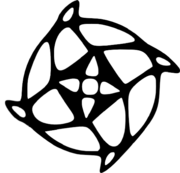
\includegraphics{bfslogosmall}
\\[4em]
{\large \bfseries Version \input{version}}
\vfill
{\Large \cc \byncsa}\\*[1em]
\emph{Licensed under Creative Commons\\*
Attribution-NonCommercial-ShareAlike License (3.0 unported).}

\end{center}
\end{titlepage}



\setcounter{secnumdepth}{-1}
\setlength{\parindent}{0cm}
\setlength{\parskip}{1.2em}

%\maketitle

\tableofcontents

\chapter[Acknowledgements]{\begin{center}Acknowledgements\end{center}}

Many thanks to those members of the Beltane Fire Society community who have created, collected and shared these games, with special thanks to Chlo\"{e} Dear and Tom Gibson for their original collections, on which this book has drawn heavily.


\chapter[Games]{\begin{center}Games\end{center}}
\pagebreak

% Include Game Files here
\begin{minipage}{\textwidth}
\game{Back to Back Introductions}{Introduction}
\play{4 or more}
\\*
Players sit in pairs, back to back.  Each pair has 3-5 minutes to chat and find out things about each other.  The group then reforms and each person has to tell the rest of the group 3-5 facts about the other person.\\*
Variations can include making the person talk for 30 seconds about the other person, or allowing the players to make up fake stories and have the group guess which parts are true/false.
\end{minipage}    \vfill

\begin{minipage}{\textwidth}
\game{Best Friend, Worst Enemy}{Warmup}
\play{4 or more}
\\*
Everyone secretly chooses a 'best friend' and 'worst enemy.  When the game starts they have to try to get as close as possible to their friend, and as far away as possible from their enemy.  After a few minutes of chaos, swap over so that your friend is your enemy and vice versa.\\*
\refer{Triangles Game}
\end{minipage}    \vfill

\begin{minipage}{\textwidth}
\game{Cat and Mouse}{Warmup}
\aka{Princess and Dragon}
\play{4 or more (an even number)}
\\*
The group is divided up into pairs, and they stand one behind the other.  One pair is split, and one person made the cat, and the other the mouse.  The cat chases the mouse (with full actions/sound effects).  If they catch them, they swap roles.  The mouse can escape from being chased by joining onto the back of one of the other pairs.  The person at the front is pushed off and becomes the cat, the original cat becoming the mouse.\\*
\end{minipage}    \vfill

\begin{minipage}{\textwidth}
\game{Chain Tig}{Tig,Warmup}
\play{8 or more}
\\*
As normal tig, except when a person is tigged they hold hands with the person who tigged them, and they both can tig people.  As more people are tigged, the chain grows longer and longer.  Only the people at the ends of the chain can tig others.
\end{minipage}    \vfill

\begin{minipage}{\textwidth}
\game{Circle Hug}{Bonding}
\aka{Ball of String}
\play{8 or more}
\\*
Everyone forms a long line, holding hands.  One person stands still and everyone else walks or runs around, winding the line up in a big hug.  (Care must be taken not to break anyone's arms!).  Once complete, the middle person crouches down and escapes out under people's arms, with the rest of the line following until it is straight again.
\end{minipage}    \vfill

\begin{minipage}{\textwidth}
\game{Circle Throw}{Introduction,Focus,Warmup}
\play{5 or more}
\equip{1 or more Balls or Short Sticks}
\\*
Everyone stand in a big circle, one person with a ball (or stick). The person with the ball must catch someone's eye and then throw the ball to them.  This continues at random around the circle.\\*
There are several variations:\\*
Once people are getting fast enough, introduce extra balls.\\*
The person with the ball must say the person's name before throwing it to them.\\*
The person must, after throwing the ball, immediately run around the circle clockwise to the next empty space.  This ends up with most people running all the time.
\end{minipage}    \vfill

\begin{minipage}{\textwidth}
\game{Dragon Tig}{Tig,Warmup}
\play{8 or more (2 teams)}
\equip{Pegs or Scarves}
\\*
Divide the group into two or more sub-groups.  Each group forms a 'conga chain' and attaches a peg or scarf to the last person's back.  Each dragon has to try to steal the peg from the other one.\\*
A variation is to have the head of each dragon try to catch its own tail.\\*
\refer{Peg Tig}
\end{minipage}    \vfill

\begin{minipage}{\textwidth}
\game{Esser Yesser}{Bonding,Focus,Ritual}
\play{4 or more}
\\*
A good way to let go of negative energy and draw positive energy back - this exercise is best not done until the group is established. Everyone stands in a circle facing in. Everyone draws in a deep breath and puts their arms above their heads. Then, altogether everyone releases the breath and flings their arms/energy in to the centre whilst saying "Esser". Then on the in-breath, they slowly draw back from the centre saying "Yesser" until they are at full stretch before releasing in to the centre with another "Esser".  this cycle repeats a few times with the intensity building each time.
\end{minipage}    \vfill

\begin{minipage}{\textwidth}
\game{Evolution}{Introduction}
\aka{Amoeba Game}
\play{5 or more}
\\*
Everyone starts moving around, pretending to be amoebas.  Whenever they bump into another player at the same 'level' they play 'rock, paper, scissors' to see who evolves, and who devolves.  Evolution goes 'Amoeba, Frog, Lizard, Rabbit, Monkey, Human' (but can be any levels you choose), acting out each creature.  The winner is whoever reaches the top level of evolution first, or the game ends when everyone becomes human.
\end{minipage}    \vfill

\begin{minipage}{\textwidth}
\game{Footlight Theatre}{Introduction,Bonding}
\play{4 or more}
\equip{}
\\*
All players sit in a circle, their feet extended and touching to make a 'stage'.  Each player has 30 seconds to stand up and talk about themselves or a subject of choice.  They must keep talking for the entire 30 seconds.
\end{minipage}    \vfill

\begin{minipage}{\textwidth}
\game{Giants, Wizards and Dwarves}{Bonding}
\play{8 or more}
\\*
The players divide into 2 teams.  Each team decides each round to be one of the three characters.  Dwarves is to crouch down, put your fingers on your head like little horns and make small noises.  Wizards stand and intone "SHA-ZAM!" whilst casting a spell. Giants hold their hands high and roar.\\*
Wizard beats Giant, Giant beats Dwarf and Dwarf beats Wizard.\\*
The two teams line up, face to face.  Both sides chant 'HO, HA, HO, HA, HO!' and then does their chosen action.  If both sides are the same, they retreat to their 'base' and decide on a new character.  If different, whichever side is the 'winner' chases the losing side, and any they catch (before they reach the safety of their 'base') join their team for the next round.  The game is over when only one team remains, or a certain number of players on one side is reached.\\*
Variations can include using different characters (e.g red, white, blue), animals (e.g cat, mouse, elephant) etc.
\end{minipage}    \vfill

\begin{minipage}{\textwidth}
\game{Granny's Footsteps}{Focus}
\play{8 or more}
\\*
One person (Granny) faces a wall with their back to the other players.  The other players line up at one end of the room and must try to sneak up on them.  Granny can turn round at any time, and the players must stand stock still. If Granny sees a player moving, they must move back to the start line.  If a player manages to touch Granny, they take over the role.\\*
For variation, Granny can wander round the room and try to put off or make laugh any of the stationary players (without touching them).\\*
\refer{Granny's Keys}
\end{minipage}    \vfill

\begin{minipage}{\textwidth}
\game{Granny's Keys}{Focus}
\play{6 or more}
\equip{Water Pistol or Small Balls, Handbag}
\\*
One person (Granny) sits on a chair, blindfolded, with a water pistol or balls, with a bunch of keys under the chair.  The other players circle round her some distance away and must try to sneak up and steal the keys.  If she hears them trying she can squirt the water pistol at them/throw a ball at them/hit them with her handbag.  Anyone who is hit has to go back to the outer circle.  If someone manages to get the keys, they become Granny.\\*
\refer{Granny's Footsteps}
\end{minipage}    \vfill

\begin{minipage}{\textwidth}
\game{Hello My Name is Joe}{Song,Warmup}
\play{1 or more}
\\*
Everyone stands in a circle, and chants the following song.  At the end of each verse a new body part is used to push the buttons, going hands, feet, head/nose and anything else you fancy!  The final verse, when asked if he is busy, he says 'Yes!'.

\begin{quote}
Hello my name is Joe!
I've got a wife and two kids and I work in the bottle factory.
One day my Boss came up to me.
He said ``Joe, are you busy?'' I said, ``No!''
He said, ``Push this button with your right hand.''
[everyone starts pushing a button with their right hand...]
\end{quote}


\end{minipage}    \vfill

\begin{minipage}{\textwidth}
\game{Hospital Tig}{Tig,Warmup}
\play{4 or more}
\equip{}
\\*
Everyone is IT and goes round trying to tig everyone else. The first time someone is tigged, they lose the use of an arm; the second time, the other arm so you have to tig with your head; then each leg and finally, the body.  Last man 'standing' wins.
\end{minipage}    \vfill

\begin{minipage}{\textwidth}
\game{Hug Tig}{Tig,Warmup}
\play{4 or more}
\equip{}
\\*
As normal tig, except that players can't be tigged if they are hugging another player.  Hugs are only allowed to last for 5 seconds, and you can't hug the same person twice, or have hugs of more than 2 people.
\end{minipage}    \vfill

\begin{minipage}{\textwidth}
\game{Monkey Song}{Song,Warmup}
\play{1 or more}
\\*
Everyone stands in a circle and sing the following song. At the point marked \textit{X}, Somebody calls out a dance move (eg ballet, tango, hip hop etc) and
 everyone does that dance or action. As each 'day' in the song progresses, the original dance plus a new one is done, until by Saturday there are 6 dances. So it continues until Sunday when the monkey is declared dead.

\begin{quote}
On Monday morning woke up late, saw a little monkey sat on me gate.\\*
So i went down to investigate, monkey was doing the latest dance craze.\\*
Monkey \textit{X}, so I \textit{X}ed too,\\*
\textit{X}, so I \textit{X}d too\\*
Ain't nothing the monkey won't do. Ain't nothing the monkey won't do.\\*

On Tuesday morning...\\*
On Wednesday morning... etc
\end{quote}


\end{minipage}    \vfill

\begin{minipage}{\textwidth}
\game{Name Games}{Introduction}
\play{5 or more}
\\*
Each player in turn says their name, going round the circle. Variations include:\\*
Alliteration - Andy likes Apples, Sarah likes Strawberries etc\\*
Shopping List - as alliteration, but each person says all the previous alliterations too - harder the more people you have!
\end{minipage}    \vfill

\begin{minipage}{\textwidth}
\game{Peg Tig}{Warmup,Tig}
\play{8 or more}
\equip{Clothes Pegs or Scraps of Material}
\\*
Attach a peg to the back of every player.  Each player must try to grab as many pegs off other players as possible.  The winner can be the 'last man standing' or the person who collects the most pegs.  Players can opt to add stolen pegs to themselves if they lose their own to stay in the game.
\end{minipage}    \vfill

\begin{minipage}{\textwidth}
\game{Points Down}{Bonding,Focus,Physical}
\play{4 or more}
\\*
The players divide up into teams of 3-5 people.  One person calls out a number, and each team has to arrange for only that many points of contact with the ground (points are head, hands, feet, bum, etc).  The group works together to reach this goal - for example with 3 people and '4' points, 2 players standing (4 feet down) can lift the other player off the ground.  Large numbers can be as hard as small ones!
\end{minipage}    \vfill

\begin{minipage}{\textwidth}
\game{Poison Pool}{Bonding}
\play{4 or more}
\\*
Everyone forms a circle holding hands, with a small area marked in the middle (about a size for one to stand in). The area is the poison pool and if you touch it then you get fatally poisoned and have to leave the circle. The idea is that as the circle moves slowly around everyone tries to throw their neighbours into the poison pool without being thrown in themselves. Last one left alive wins.
\end{minipage}    \vfill

\begin{minipage}{\textwidth}
\game{Reverse Tig}{Tig,Warmup}
\play{4 or more}
\equip{}
\\*
The opposite of standard tig: instead of trying to tig someone else by running
after them, IT tries to stay IT by avoiding being tigged by everyone else. If someone tigs IT then they become IT and everyone chases after them.  It must keep shouting 'I'm it' all the time.
\end{minipage}    \vfill

\begin{minipage}{\textwidth}
\game{Rhythm Salad}{Rhythm}
\play{4 or more}
\\*
All the players stand in a circle.  One person begins saying the name of a type of food that can be used to make a salad over and over, in a rhythmic style.  The rest of the group joins in, each picking a different food item (and accompanying rhythm).  The rhythms all mix together to make a 'rhythm salad' beat.  Players can change their item and rhythm at any time.
\end{minipage}    \vfill

\begin{minipage}{\textwidth}
\game{Roll Over}{Bonding}
\aka{Log Roll}
\play{4 or more}
\\*
Everyone lies side by side, face up. Starting at one end, each person rolls over the rest of the players, ending up face up at the far end.  The whole block moves across the ground this way.
\end{minipage}    \vfill

\begin{minipage}{\textwidth}
\game{Rubber Chicken}{Song,Warmup}
\play{1 or more}
\\*
Everyone stands in a circle. Sticking out one arm, you count down quickly from 8 to 1, shaking the arm on each count.  Repeat with the other limbs, then repeat again, this time counting from 7 down, then 6 down etc.  At the end of the last round, everyone jumps in the air and shouts 'Rubber Chicken!'
\\*
For variation, count up, start at different numbers, or count down in leaps - e.g 16x, 8x, 4x etc
\end{minipage}    \vfill

\begin{minipage}{\textwidth}
\game{Silent Cow}{Warmup}
\play{8 or more}
\\*
Everyone gets down on their hands and knees with their eyes closed.  An organiser walks round the group and secretly touches one of the players - this person is the 'Silent Cow'.  When the game starts, all the players crawl around the room.  If they bump into another player, they must say 'Moo'.  the silent cow won't moo back, and in this case the player sticks to them, also becoming silent.  Eventually everyone is joined in a lump.
\end{minipage}    \vfill

\begin{minipage}{\textwidth}
\game{Simon Says}{Bonding}
\play{4 or more}
\\*
One person is in command, and tells the others what to do (an action, movement etc).  The followers must only obey when the order is prefixed with 'Simon Says'.  Anyone following when this prefix isn't used is out.
\end{minipage}    \vfill

\begin{minipage}{\textwidth}
\game{Snake in the Grass}{Tig,Warmup}
\play{4 or more}
\\*
Mark out a small rectangle or square - no one can go outside this space. One person (the snake) lies down in the middle on their belly. Everyone else touches them with just a finger. The snake suddenly moves and tries to touch as many people as possible. Those tigged all become snakes, get down on their bellies and start trying to tig others. Pandemonium ensues until everyone is tigged.
\end{minipage}    \vfill

\begin{minipage}{\textwidth}
\game{Sticky Toffee}{Bonding}
\play{6 or more}
\\*
All but one person knots up in a heap, holding on to each other.  The person out of the heap has to try and unpick each person.  Once they have released a hand, foot, leg etc, the untangled person isn't allowed to re-use that part in tangling.  Once extracted, that person joins in trying to untangle everyone else.
\end{minipage}    \vfill

\begin{minipage}{\textwidth}
\game{Tig}{Tig,Warmup}
\aka{Catch and Tag}
\play{4 or more}
\\*
One player is 'it' and has to chase the others.  When another player is tigged, they stop, raise their arm
and shout 'I'm It'. You can play this with some places being 'wood' (like touching a tree or a wall).  Common variastions include 'safe zones' where you can't be tigged and also 'no having back' which means that if you were last IT then you can't be tigged this time.
\end{minipage}    \vfill

\begin{minipage}{\textwidth}
\game{Time Bomb Tig}{Tig,Warmup}
\aka{Toilet Tig}
\aka{Leapfrog Tig}
\play{4 or more}
\\*
As normal tig, except that players who are tigged become explosive.  they stand with their legs apart and count down slowly from 5.  If they reach zero they 'explode' and collapse to the ground, and are out of the game.  They can be 'rescued' by having another player crawl through their legs before the countdown runs out.  Players can't be tigged while crawling.\\*
Variations include Leapfrog Tig (having to leapfrog over the stuck person) and Toilet Tig (having to sit on them and pretend to use the toilet).
\end{minipage}    \vfill

\begin{minipage}{\textwidth}
\game{Triangles Game}{Focus,Warmup}
\play{6 or more}
\\*
Everyone secretly chooses two other players and tries to form an equilateral triangle with them in the space.  The whole group moves around until a stable position is found.\\*
\refer{Best Friend, Worst Enemy}
\end{minipage}    \vfill

\input{version}
\begin{minipage}{\textwidth}
\game{Zip-Zap-Boing}{Bonding, Focus}
\play{6 or more}
\\*
Everyone stands in a circle. The first person says ZIP! and points immediately either left or right makes the person left or right.  This person then continues in the same way.  After a few minutes, ZAP! is added - pointing with both hands at anyone in the circle \textit{other} than the person immediately left or right.  Thirdly, BOING! is added - throwing up your arms and 'bouncing' back a ZAP! to the sender.  Next, KER-CHING!, curving your arm over your neighborus head to the next-but-one person is added.  finally, BOING-BALOING! - 'bouncing' back a BOING! which involves both people bouncing across the circle to change spaces.\\*
When someone gets it wrong, they either leave the circle, or they crouch down and form a 'new' circle low down, whose 'losers' stand back up to the higher circle.
\end{minipage}    \vfill

\begin{minipage}{\textwidth}
\game{Zombie Name Game}{Introduction}
\play{5 or more}
\equip{}
\\*
One player begins shambling towards another, zombie-style.  The targeted player turns to another player, and makes eye contact, then says their name.  They then begin shambling towards them.  If the zombie catches the person before they start moving, they're out of the circle.
\end{minipage}    \vfill



% Output the index at the end.
\printindex{Alternatives}{Alternative Game Names}
\printindex{Index}{Categories}

\end{document}
